\documentclass[border=8pt]{standalone}
\usepackage{tikz}
\usepackage{sfmath}
\renewcommand{\familydefault}{\sfdefault}
\usetikzlibrary{arrows.meta,positioning,decorations.pathreplacing,fit,backgrounds,calc,shapes.geometric}
\definecolor{cExtract}{HTML}{2C6FB0}
\definecolor{cExtractL}{HTML}{DCE8F5}
\definecolor{cReduce}{HTML}{C77400}
\definecolor{cReduceL}{HTML}{FBE8CC}
\definecolor{cClass}{HTML}{2E7D5B}
\definecolor{cClassL}{HTML}{D8ECE2}
\definecolor{cOut}{HTML}{4A4A8A}
\definecolor{cInk}{HTML}{222222}
\tikzset{
  font=\sffamily,
  hdr/.style={rounded corners=3pt, draw=none, text=white, font=\sffamily\bfseries\small, inner sep=5pt, align=center, minimum height=8mm},
  card/.style={rounded corners=3pt, draw=#1, line width=0.8pt, fill=white, align=center, inner sep=4pt, font=\small},
  item/.style={rounded corners=2pt, draw=#1!70, fill=#1!8, align=center, font=\footnotesize, minimum width=24mm, minimum height=6mm, inner sep=2pt},
  flow/.style={-{Stealth[length=2.5mm]}, line width=0.9pt, draw=cInk},
  outb/.style={rounded corners=3pt, fill=cOut, text=white, font=\sffamily\bfseries\small, align=center, inner sep=5pt, minimum height=9mm},
}
\tikzset{
  img/.style={rounded corners=2pt, draw=cInk!60, fill=gray!12, align=center, font=\footnotesize, minimum width=14mm, minimum height=11mm, inner sep=2pt},
  proc/.style={rounded corners=3pt, draw=cExtract, line width=0.9pt, fill=cExtractL, align=center, font=\small, minimum height=9mm, inner sep=4pt},
  vecg/.style={rounded corners=3pt, draw=cClass, line width=0.9pt, fill=cClassL, align=center, font=\footnotesize, minimum height=8mm, inner sep=3pt},
  vecy/.style={rounded corners=3pt, draw=cReduce, line width=0.9pt, fill=cReduceL, align=center, font=\footnotesize, minimum height=8mm, inner sep=3pt},
  redb/.style={rounded corners=3pt, draw=cReduce, line width=0.9pt, fill=white, align=center, font=\small, minimum height=9mm, inner sep=4pt},
  clf/.style={rounded corners=3pt, draw=cClass, line width=0.9pt, fill=cClassL, align=center, font=\small, minimum height=9mm, inner sep=4pt},
  res/.style={rounded corners=3pt, fill=cOut, text=white, font=\sffamily\bfseries\footnotesize, align=center, minimum height=9mm, inner sep=4pt},
}
\tikzset{
  vstep/.style={rounded corners=3pt, line width=0.8pt, align=center, font=\footnotesize, minimum width=34mm, minimum height=8mm, inner sep=3pt},
  vflow/.style={-{Stealth[length=2mm]}, line width=0.8pt, draw=cInk},
}
\tikzset{
  vb/.style={rounded corners=3pt, line width=0.8pt, align=center, font=\scriptsize, minimum width=22mm, minimum height=7mm, inner sep=2pt},
  vw/.style={rounded corners=3pt, line width=0.8pt, align=center, font=\footnotesize, minimum width=46mm, minimum height=8mm, inner sep=3pt},
}
\newcommand{\mergeinto}[2]{% #1 = lista de nós origem (csv), #2 = nó destino
  \coordinate (by) at ([yshift=4mm]#2.north);
  \foreach \s in {#1}{\draw[line width=0.8pt,draw=cInk] (\s.south) -- (\s.south|-by);}
}

\begin{document}
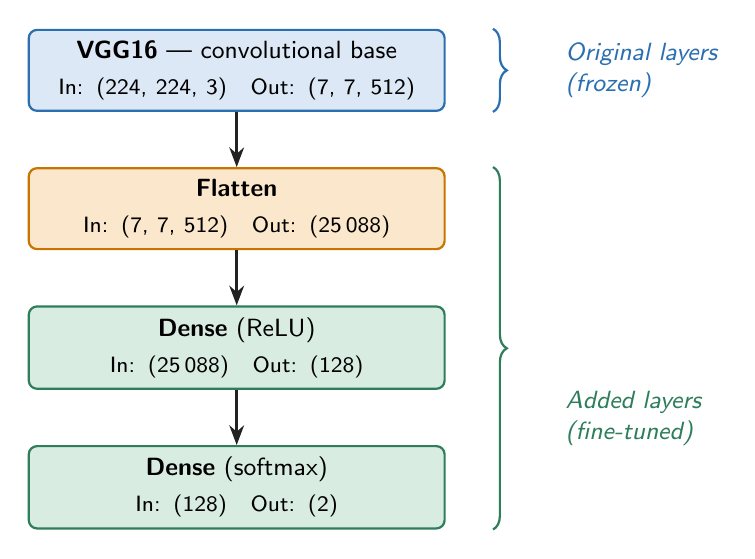
\begin{tikzpicture}[node distance=7mm]
\node[card=cExtract, text width=50mm, fill=cExtractL] (cnn)
  {\textbf{VGG16} — convolutional base\\[2pt]\footnotesize In: (224, 224, 3)\quad Out: (7, 7, 512)};
\node[card=cReduce, below=of cnn, text width=50mm, fill=cReduceL] (flat)
  {\textbf{Flatten}\\[2pt]\footnotesize In: (7, 7, 512)\quad Out: (25\,088)};
\node[card=cClass, below=of flat, text width=50mm, fill=cClassL] (d1)
  {\textbf{Dense} (ReLU)\\[2pt]\footnotesize In: (25\,088)\quad Out: (128)};
\node[card=cClass, below=of d1, text width=50mm, fill=cClassL] (d2)
  {\textbf{Dense} (softmax)\\[2pt]\footnotesize In: (128)\quad Out: (2)};
\draw[flow] (cnn)--(flat); \draw[flow] (flat)--(d1); \draw[flow] (d1)--(d2);
% brackets
\node[right=14mm of cnn, font=\small\itshape, text=cExtract, align=left] {Original layers\\(frozen)};
\draw[decorate, decoration={brace, amplitude=5pt}, draw=cExtract, line width=0.8pt] ([xshift=6mm]cnn.north east) -- ([xshift=6mm]cnn.south east);
\node[right=14mm of d1, yshift=-9mm, font=\small\itshape, text=cClass, align=left] {Added layers\\(fine-tuned)};
\draw[decorate, decoration={brace, amplitude=5pt}, draw=cClass, line width=0.8pt] ([xshift=6mm]flat.north east) -- ([xshift=6mm]d2.south east);
\end{tikzpicture}
\end{document}
